\tikzstyle{decision} = [diamond, draw, color=white,text width=4.5em, text badly centered, node distance=3.5cm, inner sep=0pt]

\tikzstyle{block} = [rectangle, draw, color=white,text width=1.5em, text centered, rounded corners, minimum height=1.5em, node distance=0.5cm,minimum height=2.25em]

\tikzstyle{hidden} = [rectangle, draw, text width=1.75em, text centered, rounded corners, minimum height=2.5em, node distance=0.6cm,minimum height=5em,fill,blue,opacity=0.85]

\tikzstyle{cloud} = [draw, color=white,ellipse, node distance=3.5cm, minimum height=2em]

\tikzstyle{line} = [draw, -latex']

\tikzstyle{MyText} = [color=white,text width=1.5cm,text centered]

\tikzstyle{vecArrow} = [color=white,thick, decoration={markings,mark=at position
	1 with {\arrow[semithick]{open triangle 60}}},
double distance=1.4pt, shorten >= 5.5pt,
preaction = {decorate},
postaction = {draw,line width=1.4pt, white,shorten >= 4.5pt}]

\tikzstyle{innerWhite} = [semithick, white,line width=1.4pt, shorten >= 4.5pt]

\tikzstyle{arrow} = [draw, -latex]

\newcommand{\smallblock}[2][0,0]{%
	\node[draw,text width=1.5em, text centered, rounded corners, minimum height=1.5em, node distance=0.5cm,minimum height=2.25em] (#2) at (#1) {#2};
}


\DeclareDocumentCommand\connector{ O{s} m O{->} m }{
	\ifthenelse{\equal{#1}{s}}{\draw[#3] (#2) -- (#4);}{}
	\ifthenelse{\equal{#1}{hv}}{\draw[#3] (#2) -| (#4);}{}
	\ifthenelse{\equal{#1}{vh}}{\draw[#3] (#2) |- (#4);}{}
	\ifthenelse{\equal{#1}{bl}}{\draw[#3] (#2) to[bend left=45] (#4);}{}
	\ifthenelse{\equal{#1}{br}}{\draw[#3] (#2) to[bend right=45] (#4);}{}
}
\section{Conversation Modeling}
%\addtocounter{framenumber}{1}

\begin{frame}{Types of Conversations}
\begin{itemize}
	\item Threaded
	\begin{itemize}
		\item Twitter, Facebook, email
	\end{itemize}
	\item Short-text conversation
	\begin{itemize}
		\item Google help desk, Microsoft Virtual Agent, etc. where the interactions are $\ge 1 < 3$
	\end{itemize}
	\item Task-oriented conversation
	\begin{itemize}
		\item Siri, Cortana, Google Home, Alexa, help desk, etc.- to get information from the user to help complete the task
	\end{itemize}
	\item Chit-chat or open conversation - unstructured conversations on any topic
	\item Question answering
\end{itemize}
\end{frame}


\begin{frame}[shrink]{Time line}
\newcommand\timeline[2]{
	\parbox[b]{8em}{\hfill{\color{cyan}\bfseries\sffamily ####1}~$\cdots\cdots$~}
	\makebox[0pt][c]{$\bullet$}\vrule\quad \parbox[c]{4.5cm}{\vspace{7pt}\color{yellow!90}\raggedright\sffamily ####2\\[7pt]}\\[-3pt]}
\centering
\begin{table}
	\begin{minipage}[t]{.7\linewidth}
		\color{gray}
		\rule{\linewidth}{1pt}
		\timeline{1950}{Turing Test}
		\timeline{1955}{AI Born}
		\timeline{1964}{ELIZA}


		\timeline{2011}{Siri}
		\timeline{2011}{IBM Watson}
		\timeline{2014}{Alexa}
		\timeline{2016}{Google Home}

		\rule{\linewidth}{1pt}
	\end{minipage}
\end{table}
\end{frame}

\subsection{Introduction}
	\begin{frame}{Conversational Modeling - Introduction}
\begin{minipage}{0.45\linewidth}
Modeling conversation is one of the active research problems in AI\\
Natural language conversation involves language understanding, reasoning, and the utilization of common sense knowledge\\
The goal is to build a conversational model that generates the responses automatically and these responses are linguistically indistinguishable from human responses thereby passing the \textit{\underline{Turing Test}}
\end{minipage}\hfill\vline\hfill
\begin{minipage}{0.5\linewidth}
	A true test for machine intelligence
	\begin{center}
	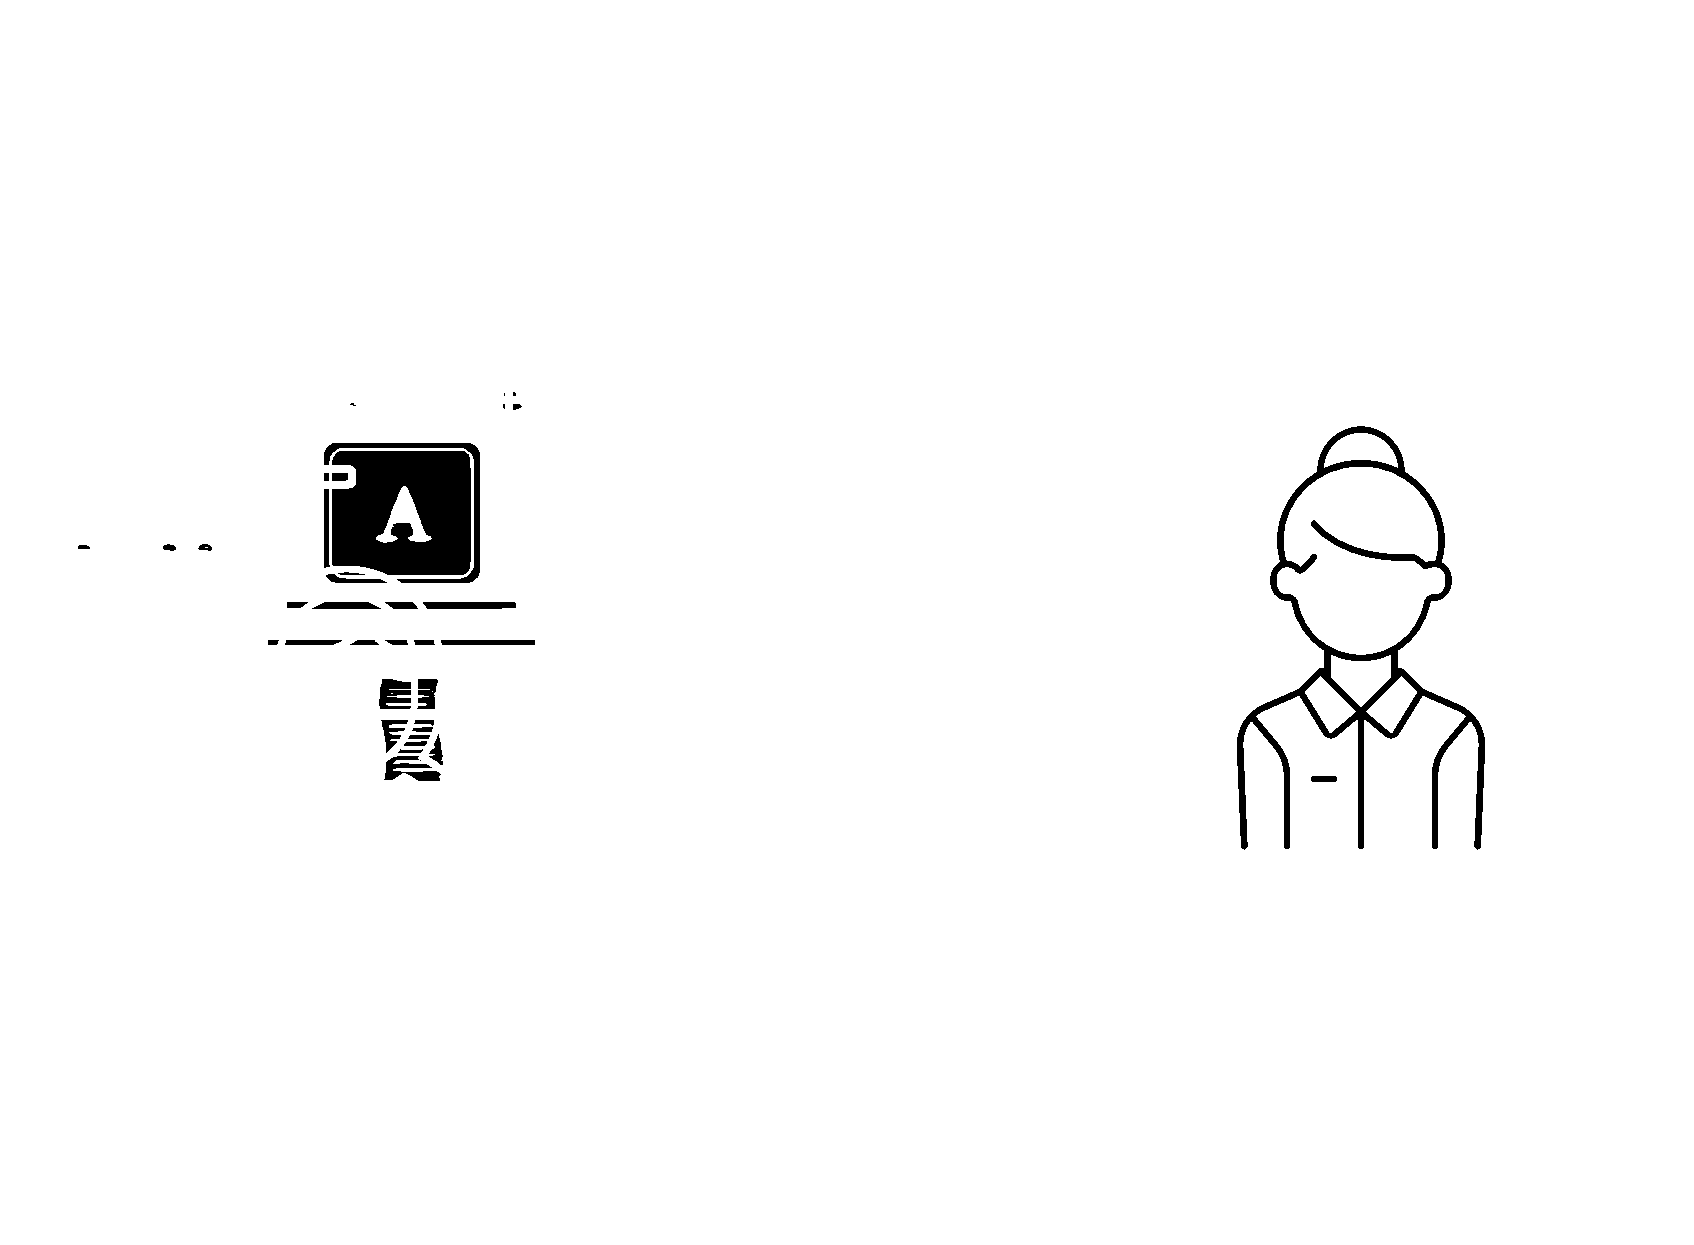
\includegraphics[width=0.7\linewidth]{./Images/TuringTest}
\end{center}
\end{minipage}
\end{frame}

\subsection{Conversation Examples}
\begin{frame}{Conversation Examples}
\begin{multicols}{2}
	\begin{description}
		\item Would you like some coffee?
		\item [*] Yes, please
		\item Mega, would you like to dance?
		\item [*] Is the floor slippery?
		\item [*]No, it's fine
	\end{description}
	\vfill
	\begin{description}
		\item [*]\textbf{Teacher}: Will you tell us the answer to question
		four?
		\item [*] \textbf{Mike}: Is that one on page (...) six or seven? Then I'd be happy to
		\item [*] \textbf{Teacher}: Six
		\item [*] \textbf{Mike}: Oh, okay. The answer is factorial two
	\end{description}
\end{multicols}

\end{frame}

\begin{frame}{Types of conversation agents}
      Chatbots and dialog-based (Google assistant, Alexa, Siri)conversational agents
    \begin{itemize}
        \item Rule-based
        \item Corpus-based
    \end{itemize}
\end{frame}
\begin{frame}{Conversation Analysis}

\begin{itemize}
\item Understanding what is \textbf{NOT }said
\item Analysis of the language beyond sentence
\item Identification of the relationship among all of the contexts across sentence boundaries
\item Consists of two parts - 	\textbf{Representation and Conditions}
\begin{enumerate}
	\item \underline{Representation} - a set of referents representing the entities which are under discussion
	\item \underline{Conditions} - a set of conditions representing the entities
	\item[] \underline{Example}
	\item[] A farmer owns a donkey
	\item[] $\left[ x,y:farmer(x),donkey(y), owns(x,y)\right]$
\end{enumerate}
\item \underline{Relationship} - how two segments of discourse are logically connected to each other
\end{itemize}

\end{frame}

%\begin{frame}{Machine Comprehension of text}
%
%\end{frame}

\subsection{Goals}
\begin{frame}{Goals of the Conversational Agent}
\begin{itemize}
\item Machine Comprehension of text
\item Learn conversations
\item Learn to summarize or encode conversation
\item Predict the meaning of the conversation
\item Produce substantiative and useful conversation
\item Produce a sentence with a good fluency
\item Detect hypocrisy, abuses, flirting, threats, etc.
\item Learn task-oriented conversation
\item Learn typical patterns of dialog discourse
\item Learn to identify questions
\item Learn Question-Answering
\end{itemize}

\end{frame}

\subsection{Examples}
\begin{frame}{ELIZA - Dr. Weizenbaum}
The first AI based conversation engine
\begin{itemize}
	\item Idea is to simulate methods used by a psychologist that involve drawing the patient out by reflecting patient's statements back at them
	\item Human-like, but does not understand the query/conversation
	\item Uses pattern matching with some rules - insertion, substitution and deletion
	\item No built in context understanding mechanism

\end{itemize}
\end{frame}

\begin{frame}{ELIZA-A Typical Conversation}
\begin{table}
	\begin{tabular}{l}
		Men are all alike. \\
		\color{yellow}IN WHAT WAY \\
		They're always bugging us about something or other. \\
		\color{yellow}CAN YOU THINK OF A SPECIFIC EXAMPLE \footnote{The capitalized conversations in {\color{yellow} yellow} are the machine responses}\\
		Well, my boyfriend made me come here. \\
		\color{yellow}YOUR BOYFRIEND MAKE YOU COME HERE \\
		he says i'm depressed much of the time. \\
		\color{yellow}I AM SORRY TO HEAR YOU ARE DEPRESSED\\
		it's me. I am not happy.\\
		\color{yellow}DO YOU  THINK    COMING  HERE WILL, HELP YOU NOT TO BE HAPPY \\
		I need some help, that much seems certain\\
		\color{yellow}WHAT WOULD IT MEAN TO YOU IF YOU GOT SOME HELP
		\footnote{Source:J.Weizenbaum, "ELIZA     A     Computer Program For the Study of Natural Language Communication Between Man And Machine",vol9, Jan. 1966  }
	\end{tabular}

\end{table}
\end{frame}


\begin{frame}[fragile]{ELIZA - How does it work - Procedure}
\begin{itemize}
	\item A text read and is inspected for the presence of a keyword
	\item If a keyword is found in the sentence, then the sentence is transformed according to a rule specified for that keyword
    \item Identification of the most important keyword in a sentence
    \item Identification of the minimal context in which the keyword occurs
    \item Choice of appropriate transformation of the input sentence by using the above using a \verb|Transformation Rule|
    \item Respond "intelligently" when there are no keywords
\end{itemize}
\begin{block}{Transform Rule}

  \begin{itemize}
      \item   \verb|User: I am very happy| $\rightarrow$ \verb|You are very happy| or \verb|How long have you been happy?|
      \item \verb|I am | $\rightarrow$ \verb|you are| - \verb|yourself| $\rightarrow$ \verb|myself| -
  \end{itemize}

\end{block}

\end{frame}

\begin{frame}{Virtual Agent - Example}
\begin{center}
	\includegraphics[width=0.7\linewidth]{"./Images/Virtual Agent - Microsoft SupportV2"}
\end{center}
\end{frame}

\begin{frame}{Question Answering - Example}
\begin{center}
	\includegraphics[width=0.55\linewidth]{"./Images/GoogleSnipetResult"}
\end{center}

\end{frame}

\begin{frame}{Jeopardy - High-level Architecture}
\begin{figure}
	\centering
	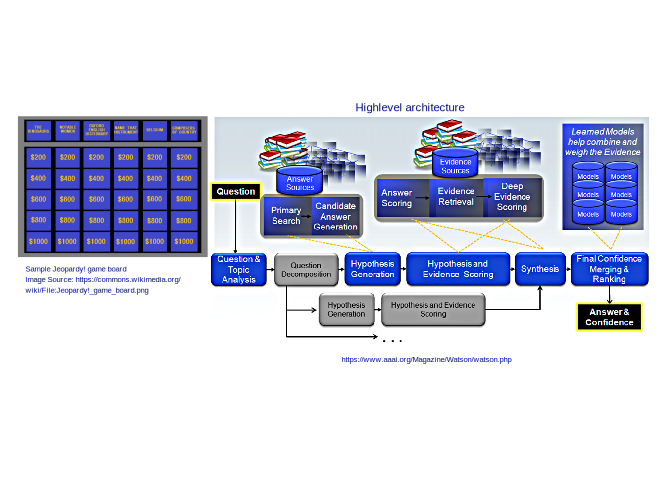
\includegraphics[width=1.0\linewidth]{./Images/Jeopardy_game_board}
	\label{fig:jeopardygameboard}
\end{figure}

\end{frame}

\begin{frame}{Historical Approach used in CM}
	\begin{itemize}
		\item Retrieval-based Approach
		\begin{itemize}
			\item Pick a suitable response based on how many times a particular response was selected for similar questions
			\item Using matching features of question and the response
			\begin{itemize}
				\item The use of matching features alone will not suffice
			\end{itemize}
		\end{itemize}
		\item Statistical Machine Translation approach
		\begin{itemize}
			\item This approach treats this as a translation problem in which the model is trained on the parallel corpus of question and response pairs
		\end{itemize}

	\end{itemize}

\end{frame}
